\documentclass{article}
\usepackage{appendix}
\usepackage{graphicx}
\usepackage{pdfpages}
\usepackage{fullpage}

\title{Architecture Reconstructing - Zeegu-Rea}
\author{Bjarke Brodin Larsen -- bjal@itu.dk}

\begin{document}
\maketitle

\section{Introduction}



\section{Methodology: tooling and process step-by-step}

In the following section I will describe which tools I 
deployed in what order and why I chose to do so.

\subsection{Getting acquainted with the system -- ChatGPT}

Because getting hints and ideas about the elephant we are attempting to 
map out is not dependent on precision and in the beginning is mostly a
text-parsing task, I utilized ChatGPT\cite{gpt4} to summarize the
contents of the repository and get an introductory idea 
(see Appendix \ref{apx:a}).
Because ChatGPT can search the web it surprised me by being adept at 
suggesting tools for further inspection which came in extremely handy!
After quickly getting some hints and a notion about what system I am dealing with,
I would normally proceed to attempt building and running the system,
this however requires me to understand and setup a back-end as well,
so I defer this until it may or may not become necessary.

\subsection{Getting an idea about what code is being touched the most -- }


\subsection{}

% npm audit?

\section{Results}


\section{Discussion}


\bibliography{lit}
\bibliographystyle{ieeetran}

\clearpage
\appendix
\section*{Appendix}

\section{ChatGPT Transcript}
\label{apx:a}
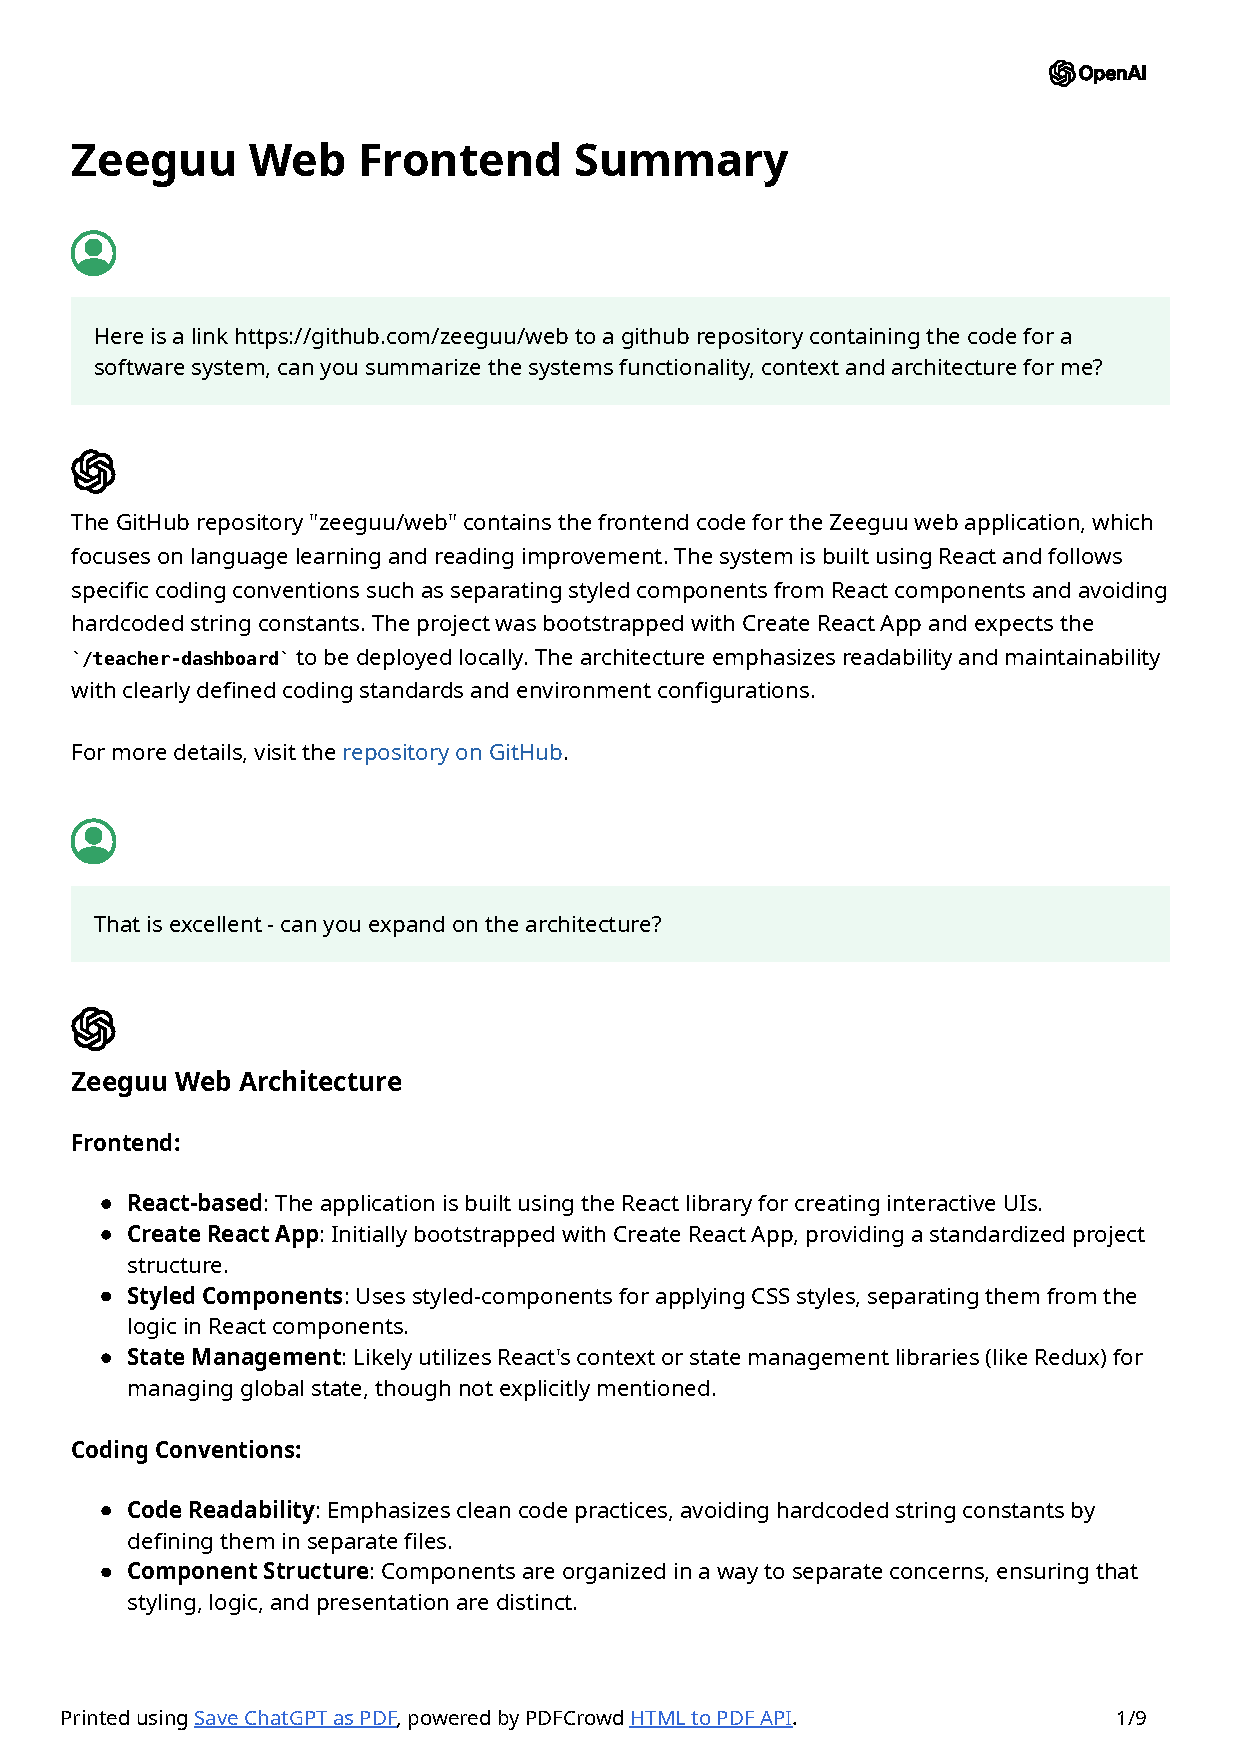
\includepdf[width=\textwidth,pages=-]{appendix/chatgpt.pdf}

\end{document}